\chapter{ROS framework}

\section{Introduction to the ROS framework}

\textbf{ROS} is an open-source robotics software framework. It is a meta-operating system, which means that it provides its own 
abstractions on top of the host's operating system including filesystem, hardware abstractions, low-level device control, 
package management and networking. It also provides tools and services to develop large, scalable 
robotics software, it supports a wide variety of libraries and programming languages and it has a huge community, support and 
documentation resources.\\


\begin{enumerate}
\item \textbf{ROS Filesystem}
\begin{itemize}
\item \textbf{Packages}
\item \textbf{Metapackages}
\item \textbf{Package Manifests}
\item \textbf{Messages}
\item \textbf{Services}
\item \textbf{Launch files}
\end{itemize}

\item \textbf{ROS Computation Graph}
\begin{itemize}
\item \textbf{Nodes}
\item \textbf{Master}
\item \textbf{Parameter Server}
\item \textbf{Topics}
\item \textbf{Bags}
\end{itemize}

\item \textbf{ROS Community}
\begin{itemize}
\item \textbf{Distributions}
\item \textbf{Repositories}
\item \textbf{ROS Wiki}
\item \textbf{ROS Answers}
\end{itemize}

\item \textbf{ROS Tools}
\begin{itemize}
\item \textbf{Gazebo}
\item \textbf{RViz}
\item \textbf{Moveit}
\item \textbf{Filesystem tools}
\end{itemize}
\end{enumerate}

\begin{center}
\begin{figure}[!htb]
\centering
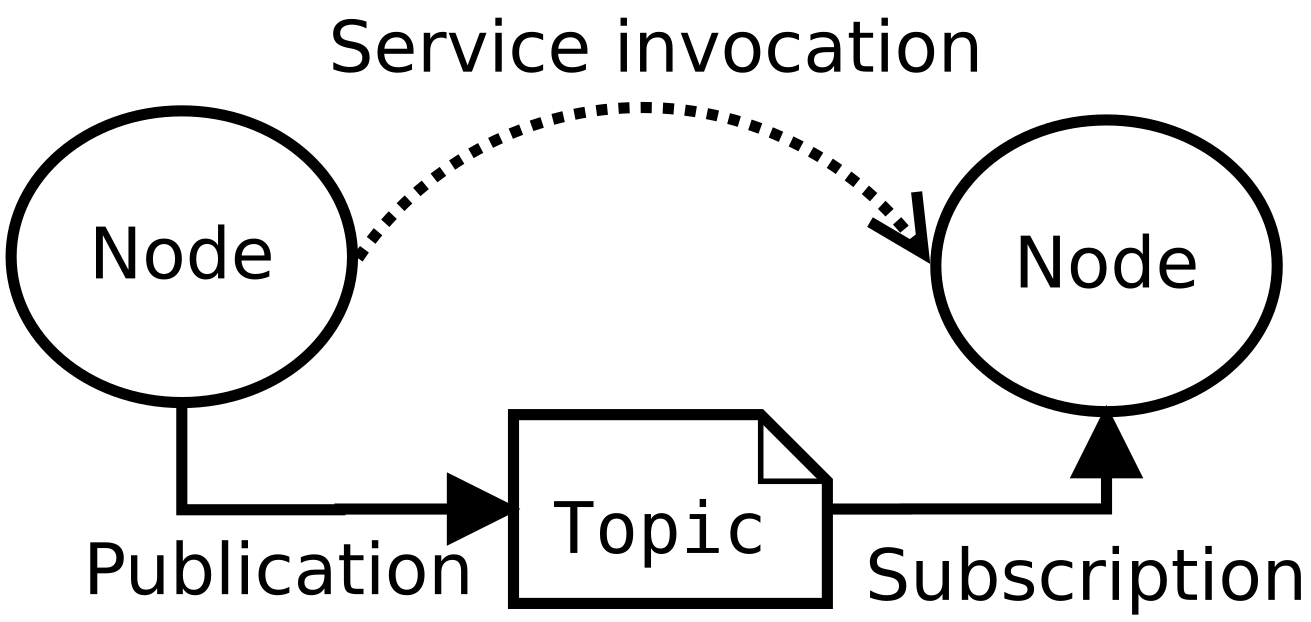
\includegraphics{images/ROS_basic_concepts_topics_nodes.png}\\
\caption{Communication diagram of 2 ROS nodes with a topic and a service}
\end{figure}
\end{center}

A \textbf{node} is a small piece of code that runs in a process and executes a task. Usually nodes should execute one task and in cases of more complex robot applications, multiple nodes are combined and run together 
to run more complicated tasks. Nodes are combined together into a graph and communicate with each other using topics, remote procedure call services and the parameter server. Splitting the robot application into multiple 
smaller nodes is more fault tolerant, because an issue or a crash in one node does not have affect much the other nodes (individual nodes are isolated). Scalability (i.e. the ability to easily add new features and code) using
nodes is also much easier, but the code complexity increases with the number of nodes, the more the number of nodes, the more the interconnections between them and the harder it is to debug issues or to run and maintain the 
nodes.\\

\textbf{Topics} are namespaced buses over which nodes exchange messages. A topic is a stream of messages with a \textbf{publish and subscribe} mechanism, which decouples the production of information from its consumption. 
Topics connect nodes in a many-to-many relationship, which means that all nodes that are interested in the topic data subscribe to the relevant topic and all nodes that generate data publish to the relevant topic. Topic data 
have a predefined \textbf{message} type that can be a String, Float, Integer, Array or even more complicated custom object structures.


\section{Gazebo simulation environment}

Gazebo \url{http://gazebosim.org/} is the most popular simulation software used in most ROS projects and it is a very important tool that mimics the real world and how the robot would realistically interact with it. It comes with a wide range of 
features such as:
\begin{itemize}
	\item Dynamics simulation with physics engines including ODE, Bullet and others, to efficiently simulate forces, torques and collisions
	\item Advanced 3D graphics utilizing OGRE that provide realistic environment rendering, lighting, shadows and textures.
	\item Sensors like 2D/3D cameras (optionally with simulated noise), laser range finders, contact sensors, force and torque sensors
	\item customizable plugins, pre-made 3D objects, environments and robots and many more
\end{itemize}

\begin{center}
\begin{figure}[!htb]
\centering
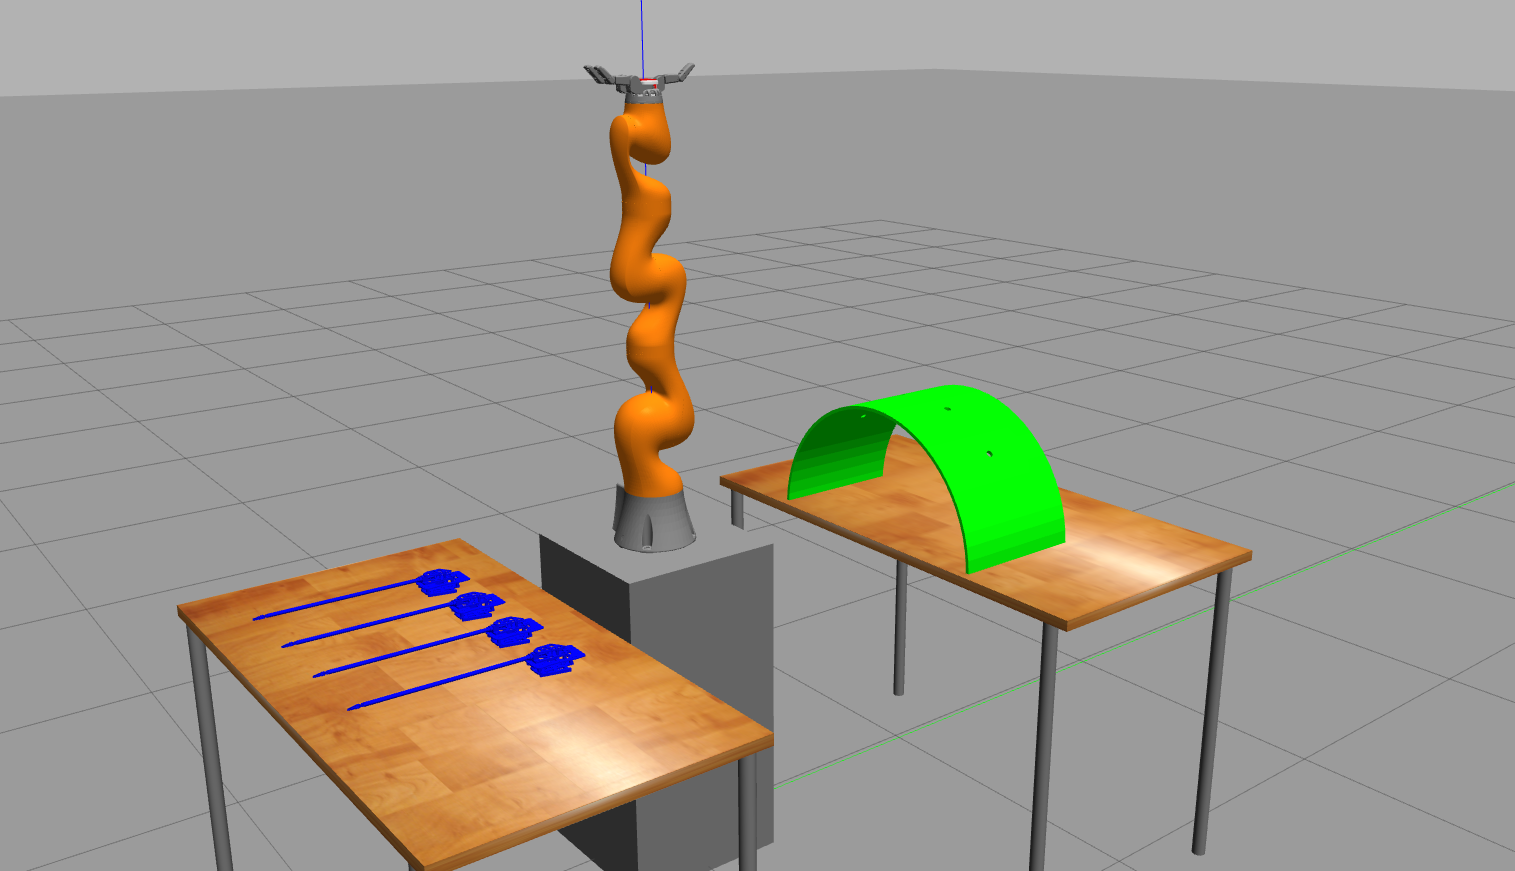
\includegraphics[width=12cm]{images/gazebo-sim1.png}\\
\caption{Simulation environment in Gazebo}
\end{figure}
\end{center}

The main environment setup of this thesis was designed using the Gazebo simulation environment and 
it consists of the following objects:
\begin{itemize}
\item the robot arm, KUKA\textsuperscript \textregistered iiwa14 lbr, being at the center of the setup
\item the robot base, so that the robot arm can better reach the tools and the surgical site and have more flexibility in movement
\item 2 tables, one for the tools and one for the surgical site
\item 4 surgical tools, using a modified version of the surgical tools used in the Raven II surgical platform
\item a mounting dock, which has holes that have the same role as the trocars (small tubes from 
which the surgical tool is inserted). Initially a mounting dock with 4 same holes of 4mm diameter was used, but it was later replaced with a new one with holes of variable diameters to test feasibility of pivot motions. Larger diameters means more space for motion planner to search for solution and thus more probable to find a solution.
\end{itemize}

\begin{center}
\begin{figure}[!htb]
\centering
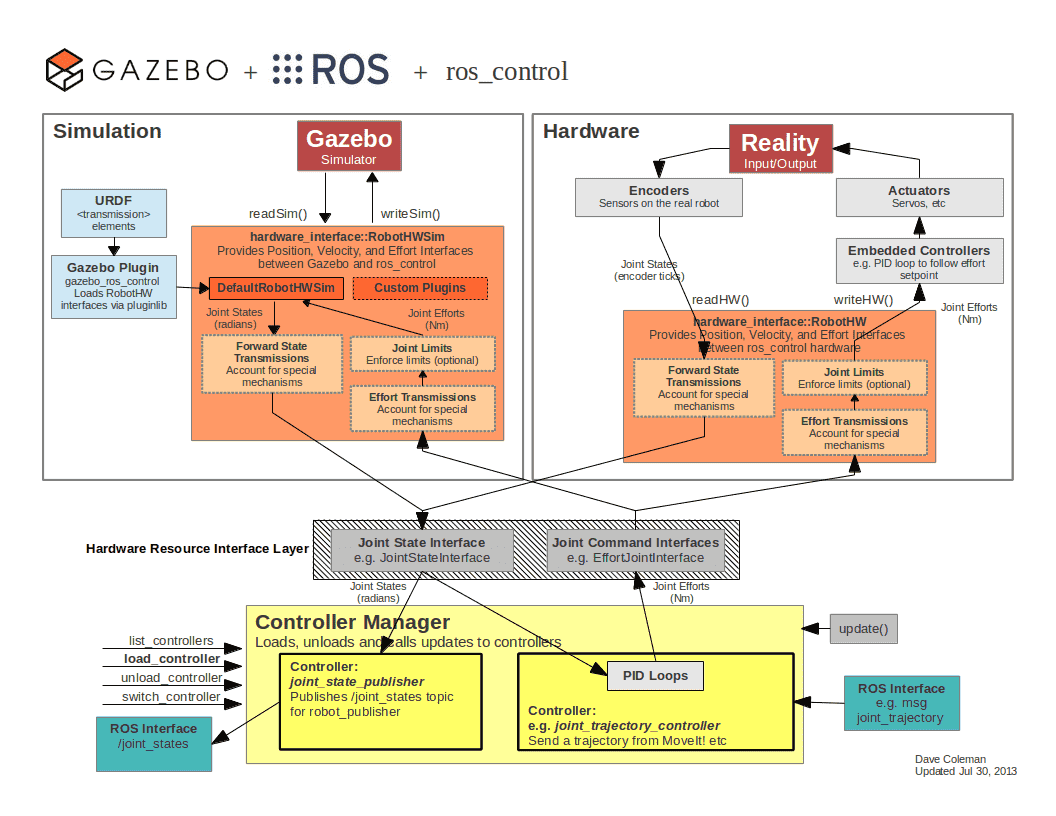
\includegraphics[width=0.6\textwidth]{images/Gazebo_ros_transmission.png}\\
\caption{Control \& Hardware Interfaces in Gazebo and ROS}
\end{figure}
\end{center}


\section{Visualization with RViz}

RViz is one of the most important and most used tools in robotic applications development and is a 3D visualizer for the Robot Operating System framework. RViz functionality should not be confused 
with that of Gazebo, because the first one visualizes the robot state and the \textbf{perceived} world (perceived objects or other calculations related to the world) whereas the second one simulates the real world.

\begin{center}
\begin{figure}[!htb]
\centering
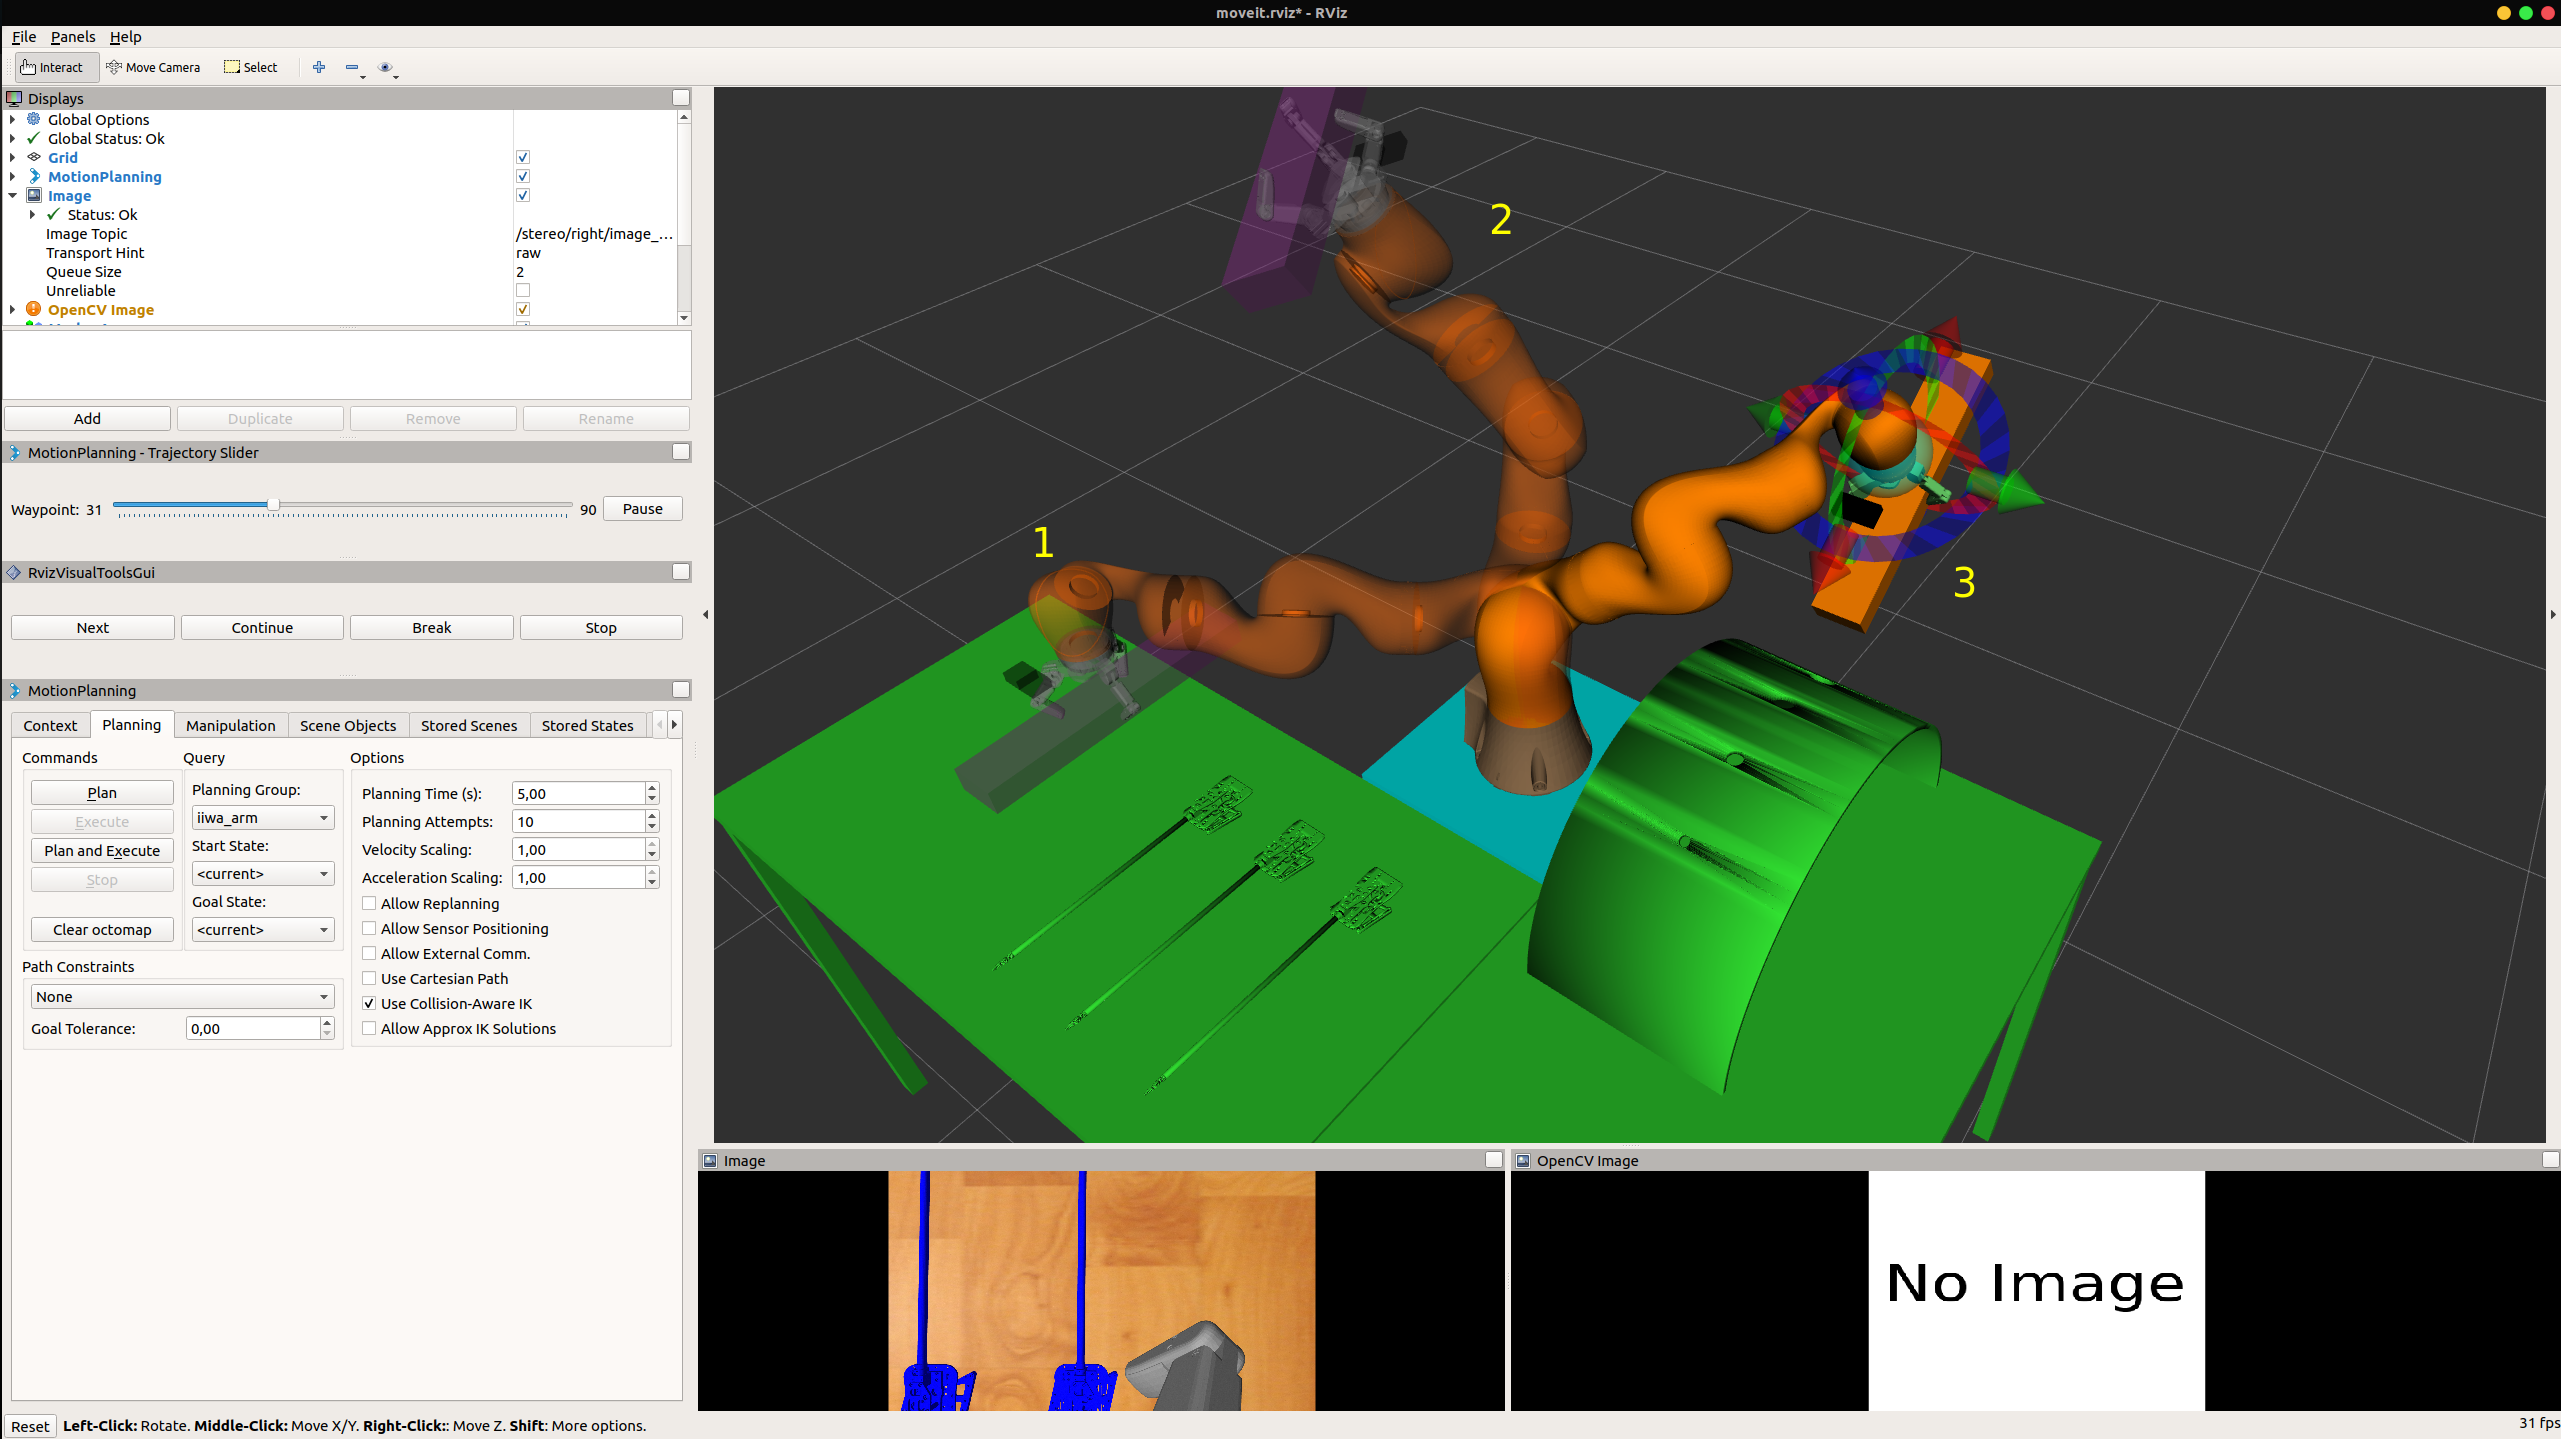
\includegraphics[width=\textwidth]{images/rviz.png}\\
\caption{RViz: Visualizing the robot state as well as the state of the perceived world\\
In this screenshot, various poses of the robot are shown: 1) the current actual real pose of the robot, 2) the planned pose and 3) the goal pose, which can 
freely be moved within the RViz environment}
\end{figure}
\end{center}

The objects that appear in RViz can either be visualized from approximations calculated from actual measurements from the robot (for example a point cloud) or can be manually loaded, in which case we make 
an assumption that the robot already "knows" the exact position, orientation, size and shape of the object, which is rarely the case in real life scenarios.
It is important to mention, that every such object is taken into consideration in collision checks and in path planning algorithms.

\section{Motion Planning with Moveit}
\label{section:moveit}

\begin{center}
\begin{figure}[!htb]
\centering
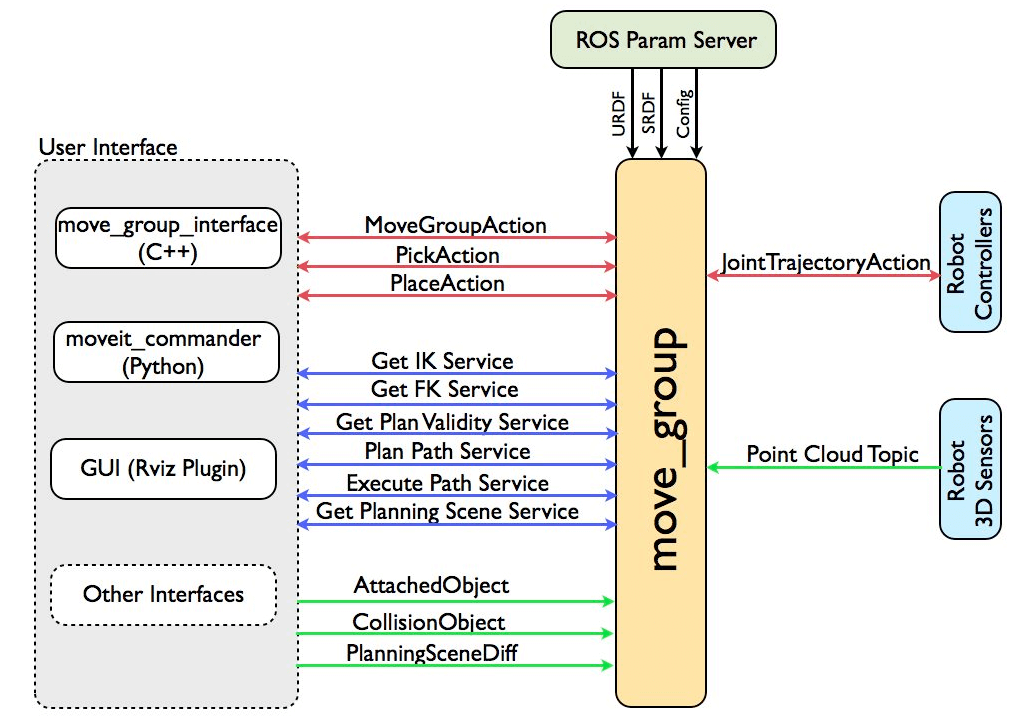
\includegraphics[width=0.6\textwidth]{images/moveit_move_group.png}\\
\caption{MoveIt ROS Architecture}
\end{figure}
\end{center}

When using the Moveit ROS library a set of parameters need to be configured in order to generate the desired commands for the controller:
\begin{itemize}
	\item \textbf{Position tolerance}: The radius of the sphere that the end-effector must reach. This is the maximum allowed error in the target's position.
	This tolerance is typically much smaller inside the surgical site, to avoid fatalities.
	\item \textbf{Orientation tolerance}: The tolerance or maximum allowed error for roll, pitch and yaw, in radians
	\item \textbf{Maximum planning time}: Maximum amount of time to be used when planning a trajectory
	\item \textbf{Replanning}: Specify whether the robot is allowed to replan if it detects changes in the environment
	\item \textbf{Maximum planning attempts}: Number of times the motion plan is to be computed from scratch before the shortest solution is returned
	\item \textbf{Base frame}: The frame in respect to which the motion plan is calculated.
	\item \textbf{Jump threshold}: This parameter sets an upper bound to the amount of "jump" (change in distance) that can occur between two consecutive trajectory points in joint 
	positions. Disabling the jump threshold while operating real hardware can cause large unpredictable motions of redundant joints 
	and could be a safety issue
	\item \textbf{Velocity scaling factor}: The approaching motion needs to be slower. We reduce the speed of the robot arm via a scaling factor of the 
	maxiumum speed of each joint. Note this is not the speed of the end effector point
	\item \textbf{End-effector step}: The resolution at which the Cartesian path is interpolated or the max step in Cartesian translation
	\item \textbf{Planner algorithm}:
	\item \textbf{Fraction}: The fraction of the path achieved as described by the waypoints
\end{itemize}

Typical motion planning parameter values outside of surgical site:
\begin{itemize}
	\item Position tolerance: 50 - 500μm
	\item Orientation tolerance: 0.00005 deg
	\item Planning time: 5-10s
	\item Replanning allowed: true
\end{itemize}

Typical motion planning parameter values inside surgical site:
\begin{itemize}
	\item Position tolerance: 5μm
	\item Orientation tolerance: 0.000005deg
	\item Planning time: 5s
	\item Replanning allowed: true
	\item End-effector interpolation step: 1mm
	\item Maximum velocity scaling factor: 0.5
	\item Maximum planning attempts: 6
\end{itemize}

Sometimes the motion planner finds a solution but the execution from the controller is aborted. 
After many iterations of the same experiment this does not happen always, which means that the 
feasibility of the execution of the movement by the controller depends on the initial state of 
the robot, i.e. if initially some joints of the robot are at their boundaries, then the next 
commanded trajectory maybe unfeasible. Another reason that the path planner may fail is the 
probabilistic nature of the path planning algorithms (see also RRT and PRM algorithms in chapter 6).

At each time step it is important to publish a custom message containing all the information 
about the kinematic state of the robot. In this thesis a custom \textbf{ROS} message was created 
containing a tf transform with a 3D vector for the position and a quaternion for the rotation and 
a custom  6-by-7 matrix containing the values of the Jacobian. The MoveIt library, from which the 
kinematic state of the robot is obtained, returns the orientation of the end effector as a 3-by-3 
rotation matrix, but in the ROS tf message it must be expressed as a quaternion. To convert the 
matrix to a quaternion we first calculate the euler angles and then use these values to construct 
the quaternion “vector”. The quaternion representation of rotation is often preferred in robotic 
applications due to its efficiency in calculations and memory. To convert the transformation 
matrix to euler angles and then to quaternions the following formulas were used:
\[
T = 
\begin{bmatrix}
r_{11} & r_{12} & r_{13} & x \\
r_{21} & r_{22} & r_{23} & y \\
r_{31} & r_{32} & r_{33} & z \\
0 & 0 & 0 & 1\\
\end{bmatrix}
\]

\[
φ = atan2(r_{21}, r_{11})
\]

\[
θ = atan2(-r_{31}, \sqrt{r_{11}^2 + r_{21}^2})
\]

\[
ψ = atan2(r_{32}, r_{33})
\]

where $T$ is the transformation matrix and $φ, θ, ψ$ are the roll, pitch and yaw (Euler) angles.


\section{Tools, Packages and Libraries}

\begin{itemize}
	\item \textbf{moveit} libraries for path planning and kinematics solutions (see more in \ref{section:moveit}). More specifically the following libraries, among others, were used 
	moveit\_core, moveit\_ros\_planning\_interface, moveit\_ros\_planning, moveit\_visual\_tools
	\item \textbf{tf2} is an important library that allows to keep track of multiple coordinate frames over time as well as calculate poses with respect to a given reference frame and apply
	transformations to vectors or other transformations (see more in bibliography in \cite{6556373} or at \url{http://wiki.ros.org/tf2}).
	\item \textbf{geometry\_msgs}: used mostly for the Pose and PoseWithCovarianceStamped messages to exchange robot and object poses between nodes and give them as input to moveit's path planners
	\item \textbf{Eigen}: a c++ library to efficiently do linear algebra calculations (matrix multiplications, inversions, vector calculations and simple geometrix calculations like finding the distance between a line and a 
	point)
	\item \textbf{OpenCV2} together with the \textbf{cv\_bridge} ROS package for the computer vision tasks of this thesis
	\item \textbf{numpy}
	\item Stereo Vision with \textbf{stereo\_image\_proc}
	\item State machines with \textbf{Smach}
	\item \textbf{actionlib}
	\item \textbf{barrett\_hand} \url{https://github.com/RobotnikAutomation/barrett\_hand.git}
	\item \textbf{gazebo-pkgs} \url{https://github.com/JenniferBuehler/gazebo-pkgs.git}
	\item \textbf{moveit-pkgs} \url{https://github.com/JenniferBuehler/moveit-pkgs.git}
	\item \textbf{general-message-pkgs} \url{https://github.com/JenniferBuehler/general-message-pkgs.git}
\end{itemize}